\documentclass{article}

\usepackage[utf8]{inputenc}
\usepackage{graphicx}


\begin{document}

\title{Identity Management on GitHub}
\author{Marco Brack \and Carsten Hartenfels \and Michael Monschau}
\maketitle

\begin{abstract}
  Lorem ipsum dolor sit amet, consectetur adipisicing elit, sed do eiusmod tempor incididunt ut labore et dolore magna aliqua. Ut enim ad minim veniam, quis nostrud exercitation ullamco laboris nisi ut aliquip ex ea commodo consequat. Duis aute irure dolor in reprehenderit in voluptate velit esse cillum dolore eu fugiat nulla pariatur. Excepteur sint occaecat cupidatat non proident, sunt in culpa qui officia deserunt mollit anim id est laborum.
\end{abstract}

\section{Introduction}

Lorem ipsum dolor sit amet, consectetur adipisicing elit, sed do eiusmod tempor incididunt ut labore et dolore magna aliqua \cite{goeminne2013comparison}. Ut enim ad minim veniam, quis nostrud exercitation ullamco laboris nisi ut aliquip ex ea commodo consequat. Duis aute irure dolor in reprehenderit in voluptate velit esse cillum dolore eu fugiat nulla pariatur. Excepteur sint occaecat cupidatat non proident, sunt in culpa qui officia deserunt mollit anim id est laborum.

Lorem ipsum dolor sit amet, consectetur adipisicing elit, sed do eiusmod tempor incididunt ut labore et dolore magna aliqua. Ut enim ad minim veniam, quis nostrud exercitation ullamco laboris nisi ut aliquip ex ea commodo consequat. Duis aute irure dolor in reprehenderit in voluptate velit esse cillum dolore eu fugiat nulla pariatur. Excepteur sint occaecat cupidatat non proident, sunt in culpa qui officia deserunt mollit anim id est laborum.

This can be seen in figure \ref{fig:graph-django-oscar}.

\section{Related Work}
\section{Identity Management}
\section{Validation}
\section{Results}

\bibliography{paper}
\bibliographystyle{plain}

\clearpage
\appendix
\section{Figures}

\begin{figure}[h]
  \centering
  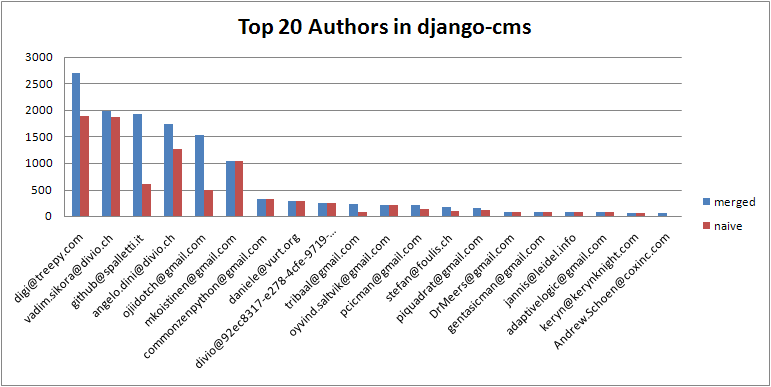
\includegraphics[width=1\textwidth]{../presentation/img/graph-django-cms.png}
  \caption{The graph for django-cms, man.}
  \label{fig:graph-django-cms}
\end{figure}

\begin{figure}[h]
  \centering
  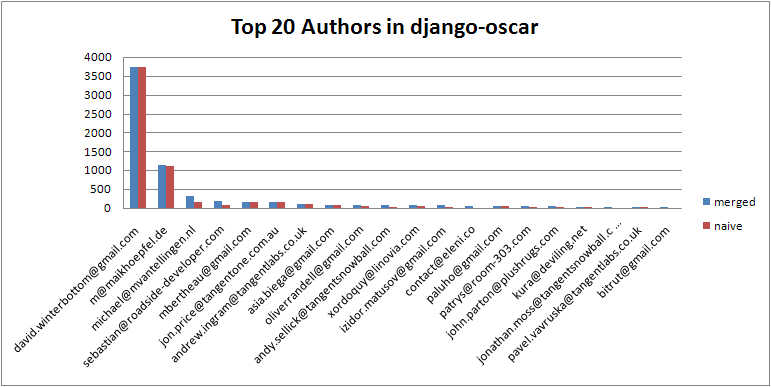
\includegraphics[width=1\textwidth]{../presentation/img/graph-django-oscar.png}
  \caption{The graph for django-oscar, man.}
  \label{fig:graph-django-oscar}
\end{figure}

\begin{figure}[h]
  \centering
  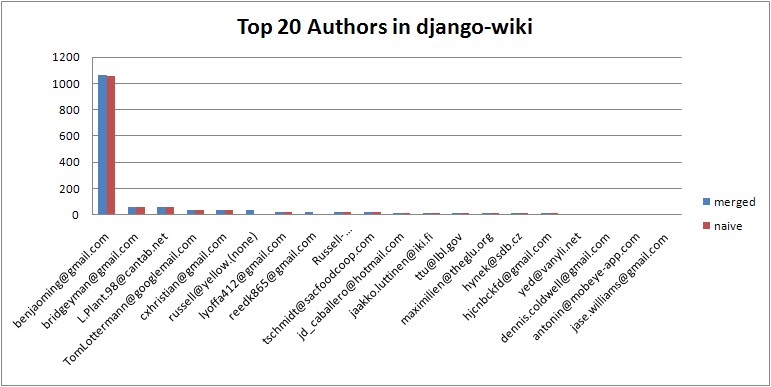
\includegraphics[width=1\textwidth]{../presentation/img/graph-django-wiki.png}
  \caption{The graph for django-wiki, man.}
  \label{fig:graph-django-wiki}
\end{figure}

\begin{figure}[h]
  \centering
  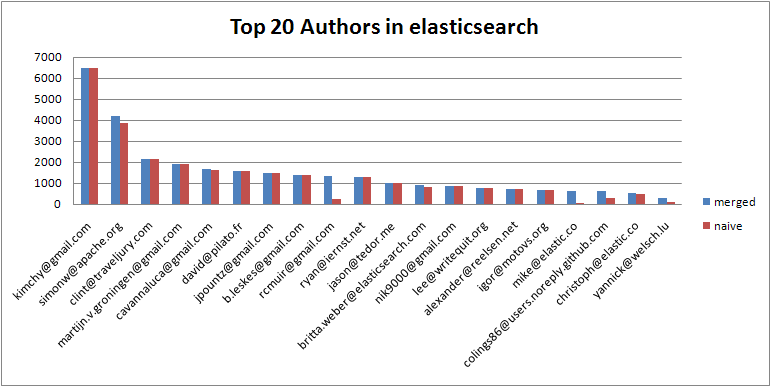
\includegraphics[width=1\textwidth]{../presentation/img/graph-elasticsearch.png}
  \caption{The graph for elasticsearch, man.}
  \label{fig:graph-elasticsearch}
\end{figure}

\begin{figure}[h]
  \centering
  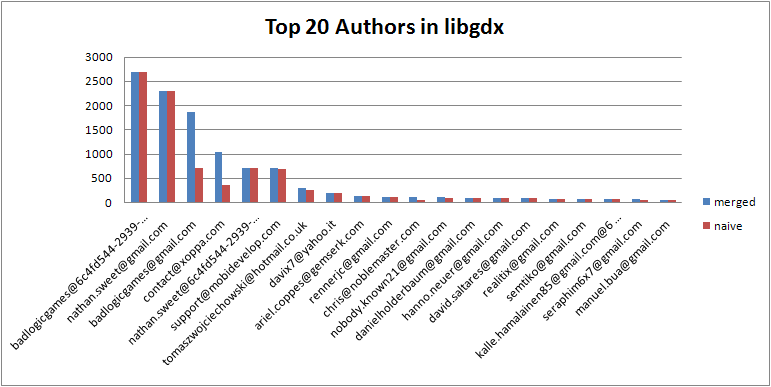
\includegraphics[width=1\textwidth]{../presentation/img/graph-libgdx.png}
  \caption{The graph for libgdx, man.}
  \label{fig:graph-libgdx}
\end{figure}

\begin{figure}[h]
  \centering
  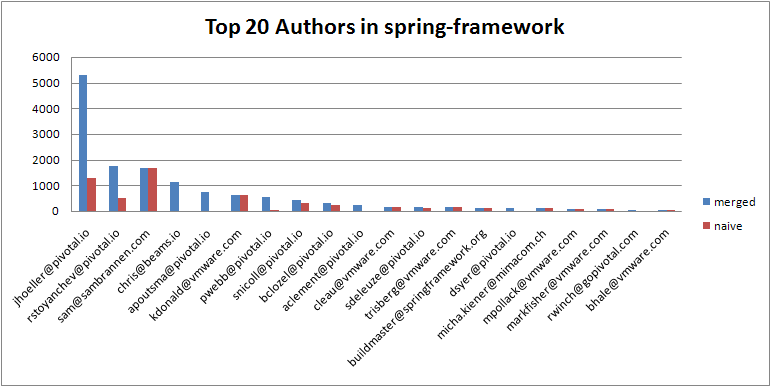
\includegraphics[width=1\textwidth]{../presentation/img/graph-spring-framework.png}
  \caption{The graph for spring-framework, man.}
  \label{fig:graph-spring-framework}
\end{figure}

\end{document}
